\section{模型准备}

为了后续模型的建立与求解,本文进行如下模型准备,即数据清洗、数据量化等。具体机制如\cref{fig:模型准备机制}所示。

\begin{figure}[h!]
\centering
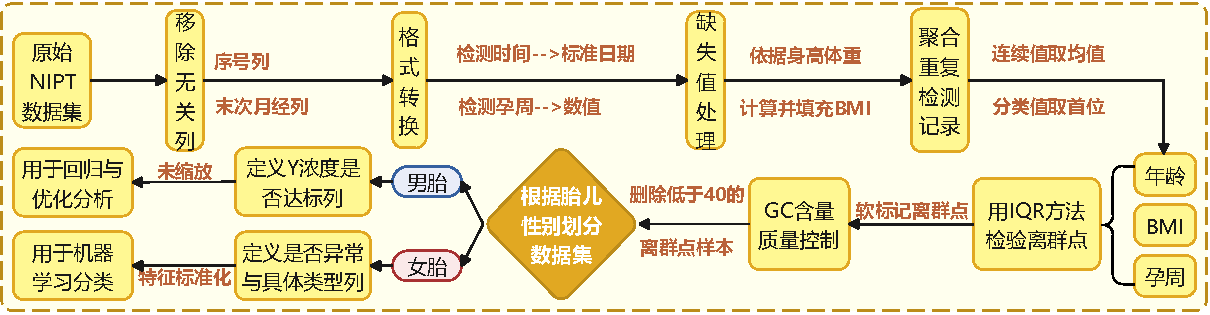
\includegraphics[width=1\textwidth]{figs/2模型准备/模型准备.pdf}
\caption{模型准备机制}
\label{fig:模型准备机制}
\end{figure}

\subsection{数据清洗}

\subsubsection{缺失值处理与数据整合}
为简化数据集,我们移除了与建模任务无直接关联的序号列。随后,我们对数据集中各变量进行缺失值统计,发现末次月经时间列存在部分数据缺失。末次月经时间的主要功能为推算孕周,而数据集中已包含更为直接的检测孕周列,故将其移除。

为使原始特征能够用于定量分析,我们需要将其转化为标准的数值格式。对于纯数字格式的检测时间列,我们将其转换为标准的日期时间格式;对于文本格式的检测孕周列,我们转换为可计算的浮点数值,例如十二周加三天转化为12.43周。对于孕妇BMI指标列中的缺失值,我们利用同一条记录的身高与体重数据,依据身体质量指数的官方计算公式进行填充,该公式如下所示
\begin{equation}
BMI = \frac{Weight(kg)}{Height(m)^2}
\label{eq:bmi}
\end{equation}
与使用均值或中位数等统计量填充相比,利用已有数据进行计算能最大限度地保持数据的真实性。



完成基础清洗与计算后,数据集内核心特征的整体分布如\cref{fig:核心特征分布}所示。该图展示了孕妇年龄,孕妇BMI与检测孕周三个变量的分布状况。从图中可以看出样本的年龄主要集中在25至35岁之间,孕妇BMI分布的峰值位于30附近,证实了样本多为高BMI的地区特征。检测孕周则在12至25周之间呈现多个峰值,表明了检测时间点的集中性。

\begin{figure}[h!]
\centering
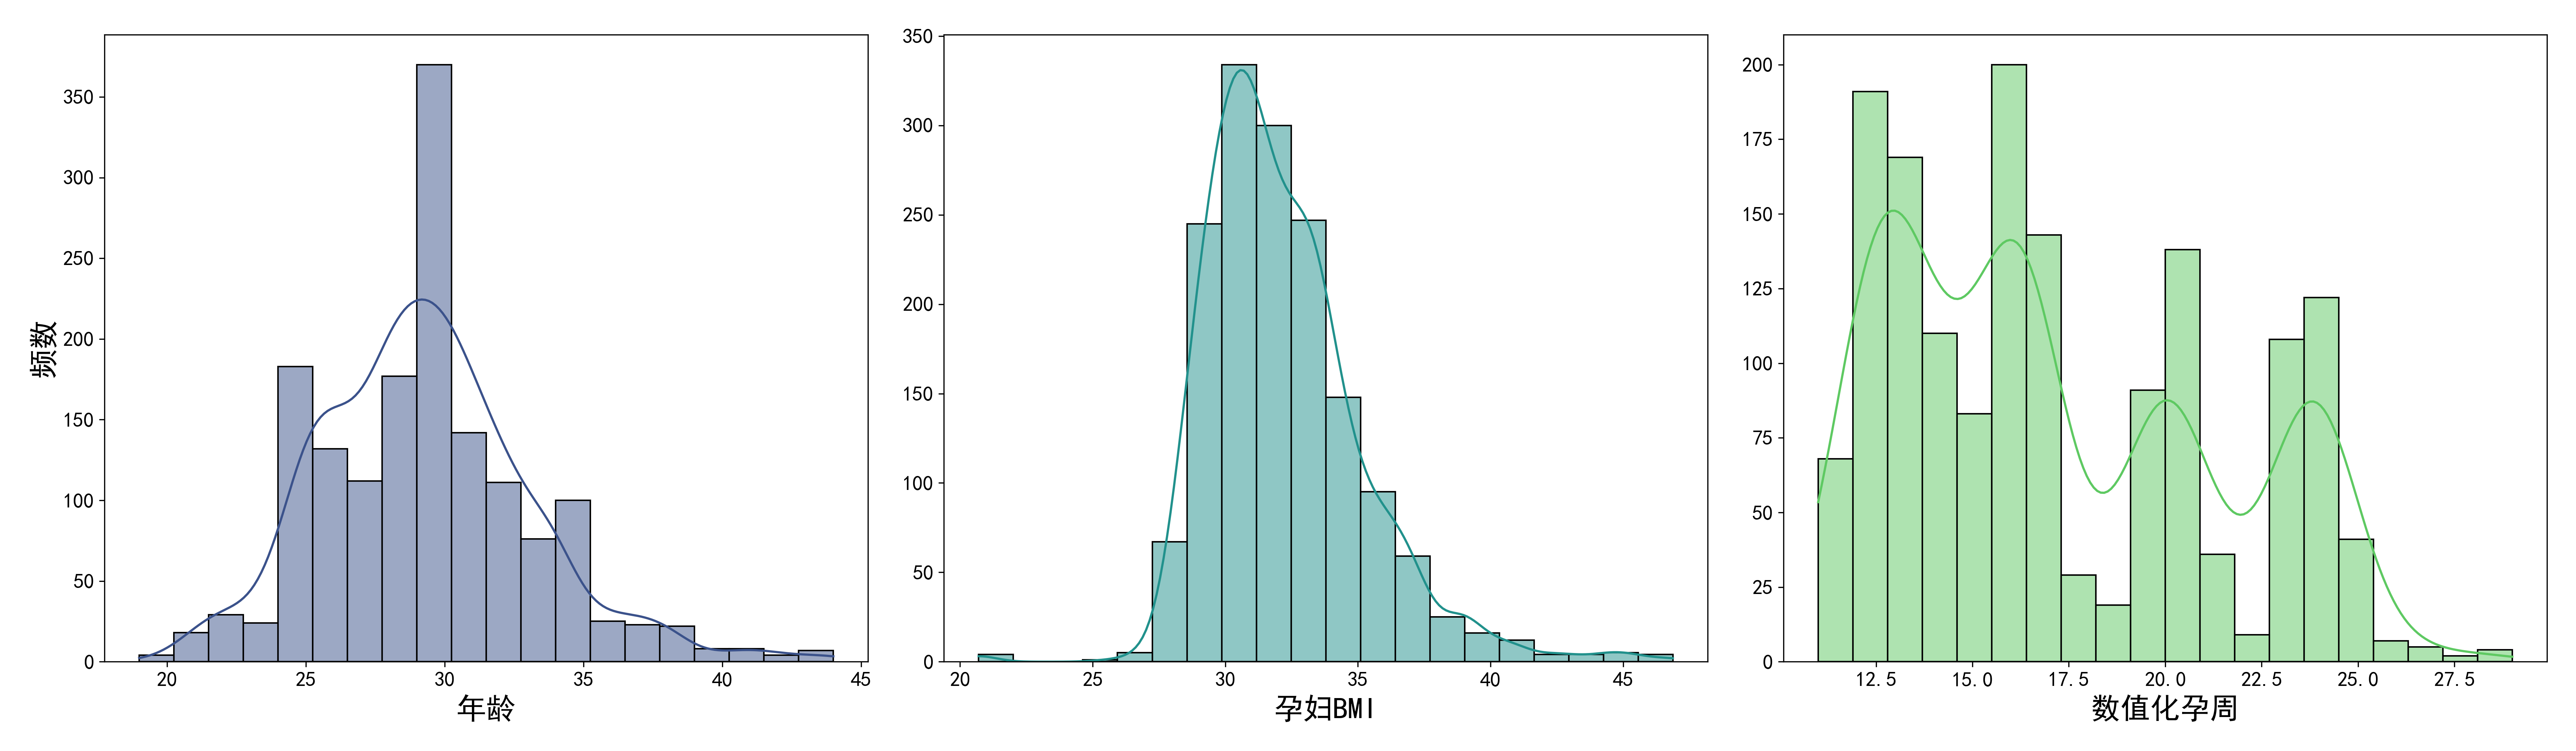
\includegraphics[width=1\textwidth]{figs/2模型准备/图1_核心特征分布.png}
\caption{核心特征分布}
\label{fig:核心特征分布}
\end{figure}

题目中提到存在对同一孕妇进行重复检测的情况,这导致了数据冗余。为消除此冗余,我们以孕妇代码与检测抽血次数为唯一标识,对同一抽血样本的多次检测记录进行数据整合。整合时,对于连续性测量指标,取其算术平均值以减小单次测量的随机误差影响;对于分类性状态指标,则保留其首次出现的值。

\cref{fig:整合效果对比}展示了数据整合前后的样本数量变化。如左图所示,处理前单个孕妇的样本记录数最高可达9条,多数孕妇具有1至6条记录。经过整合处理后,转变为每次抽血对应唯一记录的形式。如右图所示,单个孕妇的有效检测次数减少至1至5次,大部分孕妇只有4次有效检测,从而消除了冗余信息。

根据题目说明,原始数据中存在同一孕妇多次采血多次检测或一次采血多次检测的情况,这种情况造成了数据冗余。为消除此冗余并为每个样本建立唯一的检测记录,本文以孕妇代码与检测抽血次数的组合为标识,对重复的检测条目进行聚合处理。在聚合过程中,对于连续型测量指标,采用算术平均值以平滑单次测量的随机波动。对于分类性质的状态指标,则保留其初次记录的值。

该聚合过程的效果通过\cref{fig:整合效果对比}中的前后对比得以展示。左图显示在处理前,单个孕妇对应的所有样本的所有检测记录数从1条至9条不等,其中多数孕妇具有3至6条记录。经过聚合处理后,如右图所示,每位孕妇的有效检测次数范围缩小至1至5次,其中具有4次有效检测的孕妇数量最多。


\begin{figure}[h!]
    \centering
    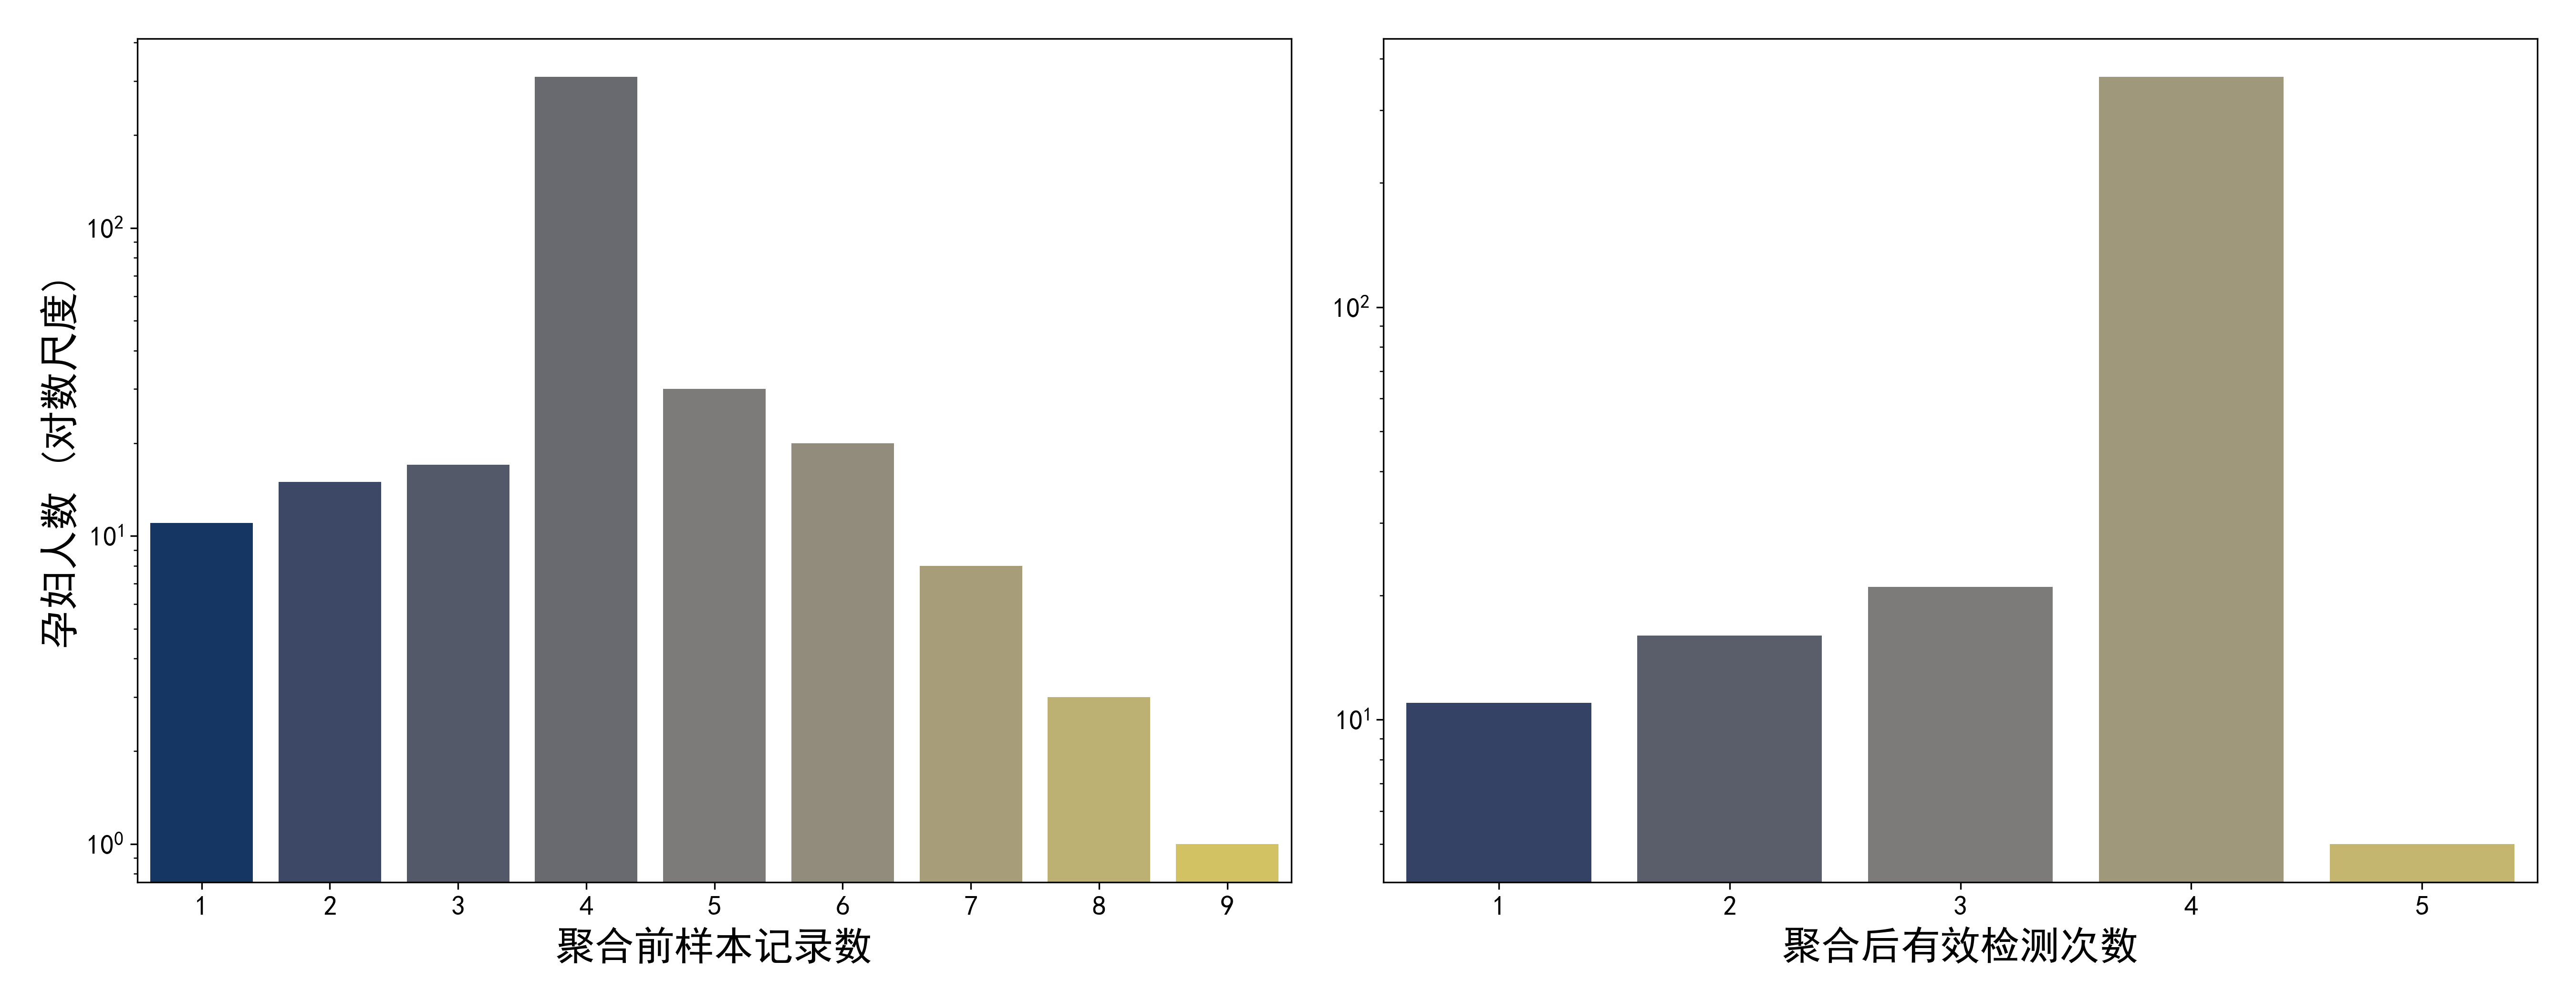
\includegraphics[width=1\textwidth]{figs/2模型准备/图2_聚合效果对比.png}
    \caption{数据整合效果对比}
    \label{fig:整合效果对比}
\end{figure}

\subsubsection{异常值处理}

我们首先针对年龄,孕妇BMI与孕周这三个核心特征执行四分位距法检验。对于识别出的离群点,本文采用软标记方法,即在数据集中新增一列用以标记样本是否为离群点,而不直接删除样本记录。离群点可能代表了真实存在的极端生理状况或数据录入错误,采用软标记策略为后续建模提供了灵活性。\cref{fig:IQR离群点分析}展示了离群点分析的过程,图中每个子图的小提琴形状表示了数据的分布,红色的圆点则标记出被标准四分位距准则判定为离群点的样本。图中可见,年龄的离群点主要分布在40岁以上的高龄区间,孕妇BMI的离群点则同时出现在低于20的低值区域与高于40的高值区域,而孕周的离群点相对较少。

\begin{figure}[h!]
\centering
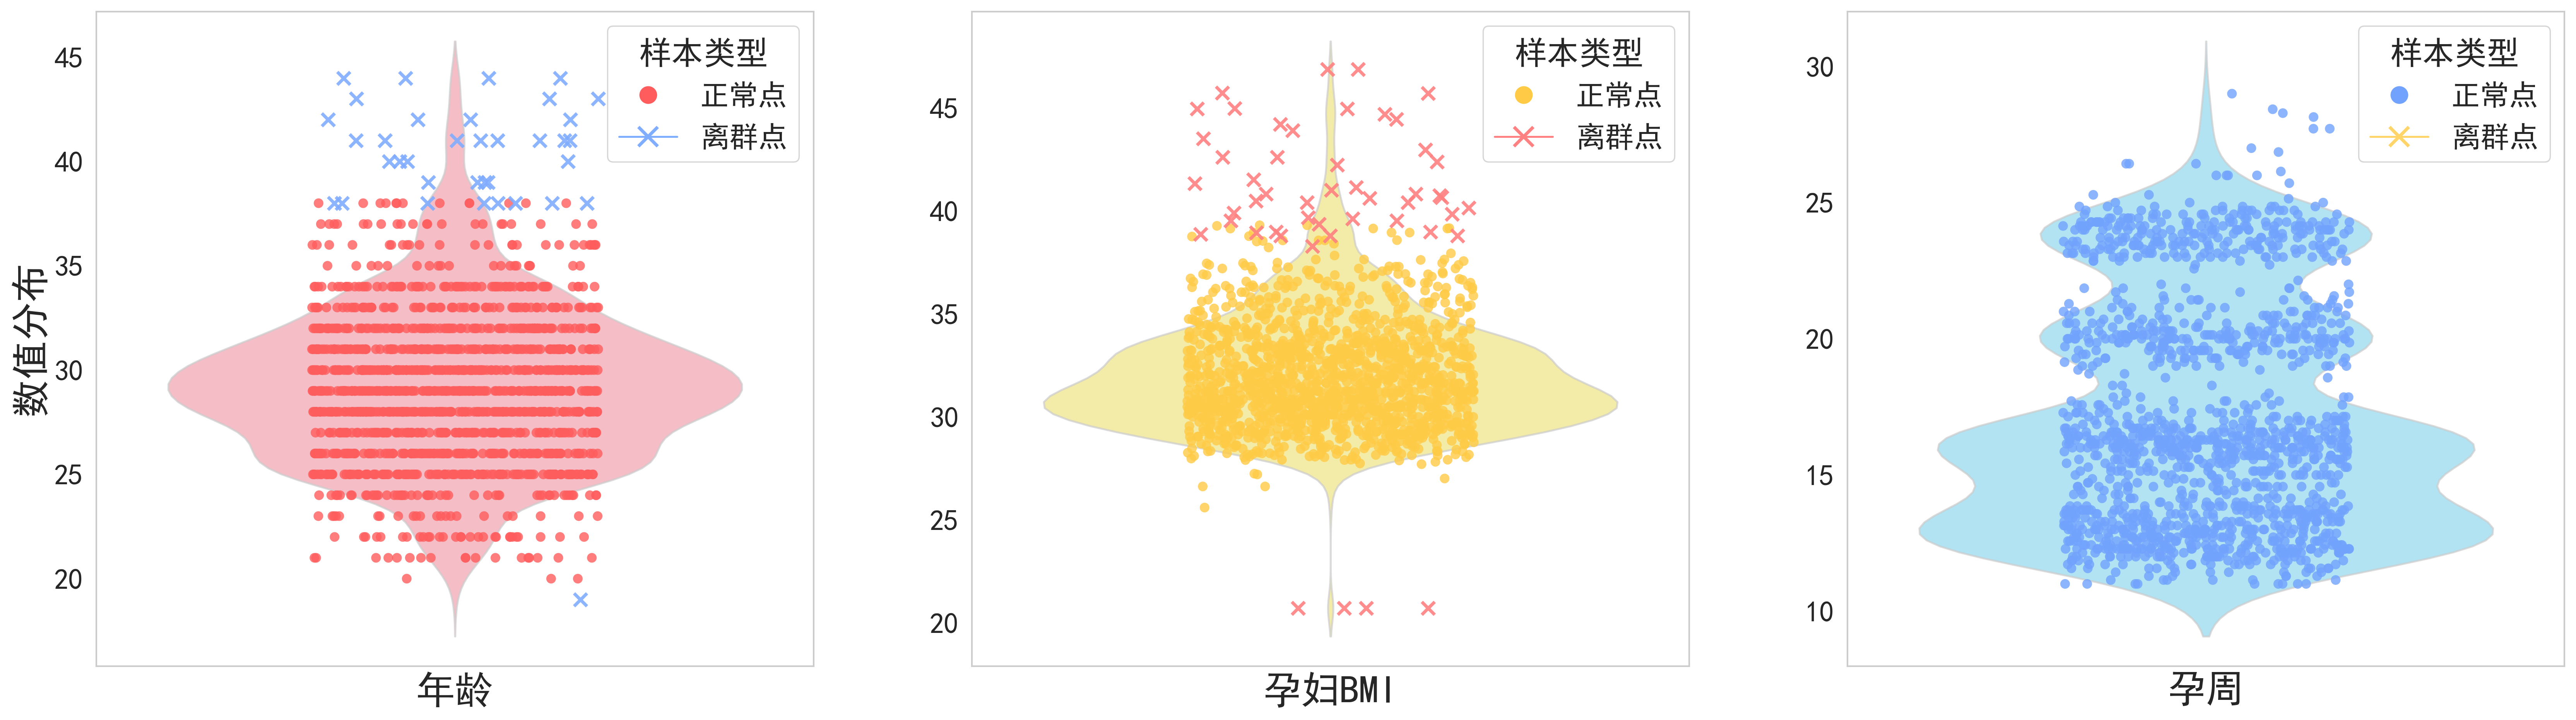
\includegraphics[width=1\textwidth]{figs/2模型准备/图3_IQR离群点分析.png}
\caption{IQR离群点分析}
\label{fig:IQR离群点分析}
\end{figure}

其次我们对GC含量进行质量控制。GC含量是衡量测序质量的重要指标。处理过程结合了统计学检验与业务规则,先对GC含量列执行标准的1.5倍四分位距检验以识别出所有统计学上的离群点。然后,仅将这些离群点中数值低于40\%的样本从数据集中直接删除。此方法能够剔除那些不仅在统计上异常,且低于业务经验常规下限的低质量测序样本。\cref{fig:GC含量离群点分析}展示了处理后的数据,其中直方图展示了GC含量的整体分布形态近似正态分布,频数在0.400处达到峰值,绝大多数样本的GC含量分布在0.395至0.405之间,分布集中,数据质量较高。

\begin{figure}[h!]
\centering
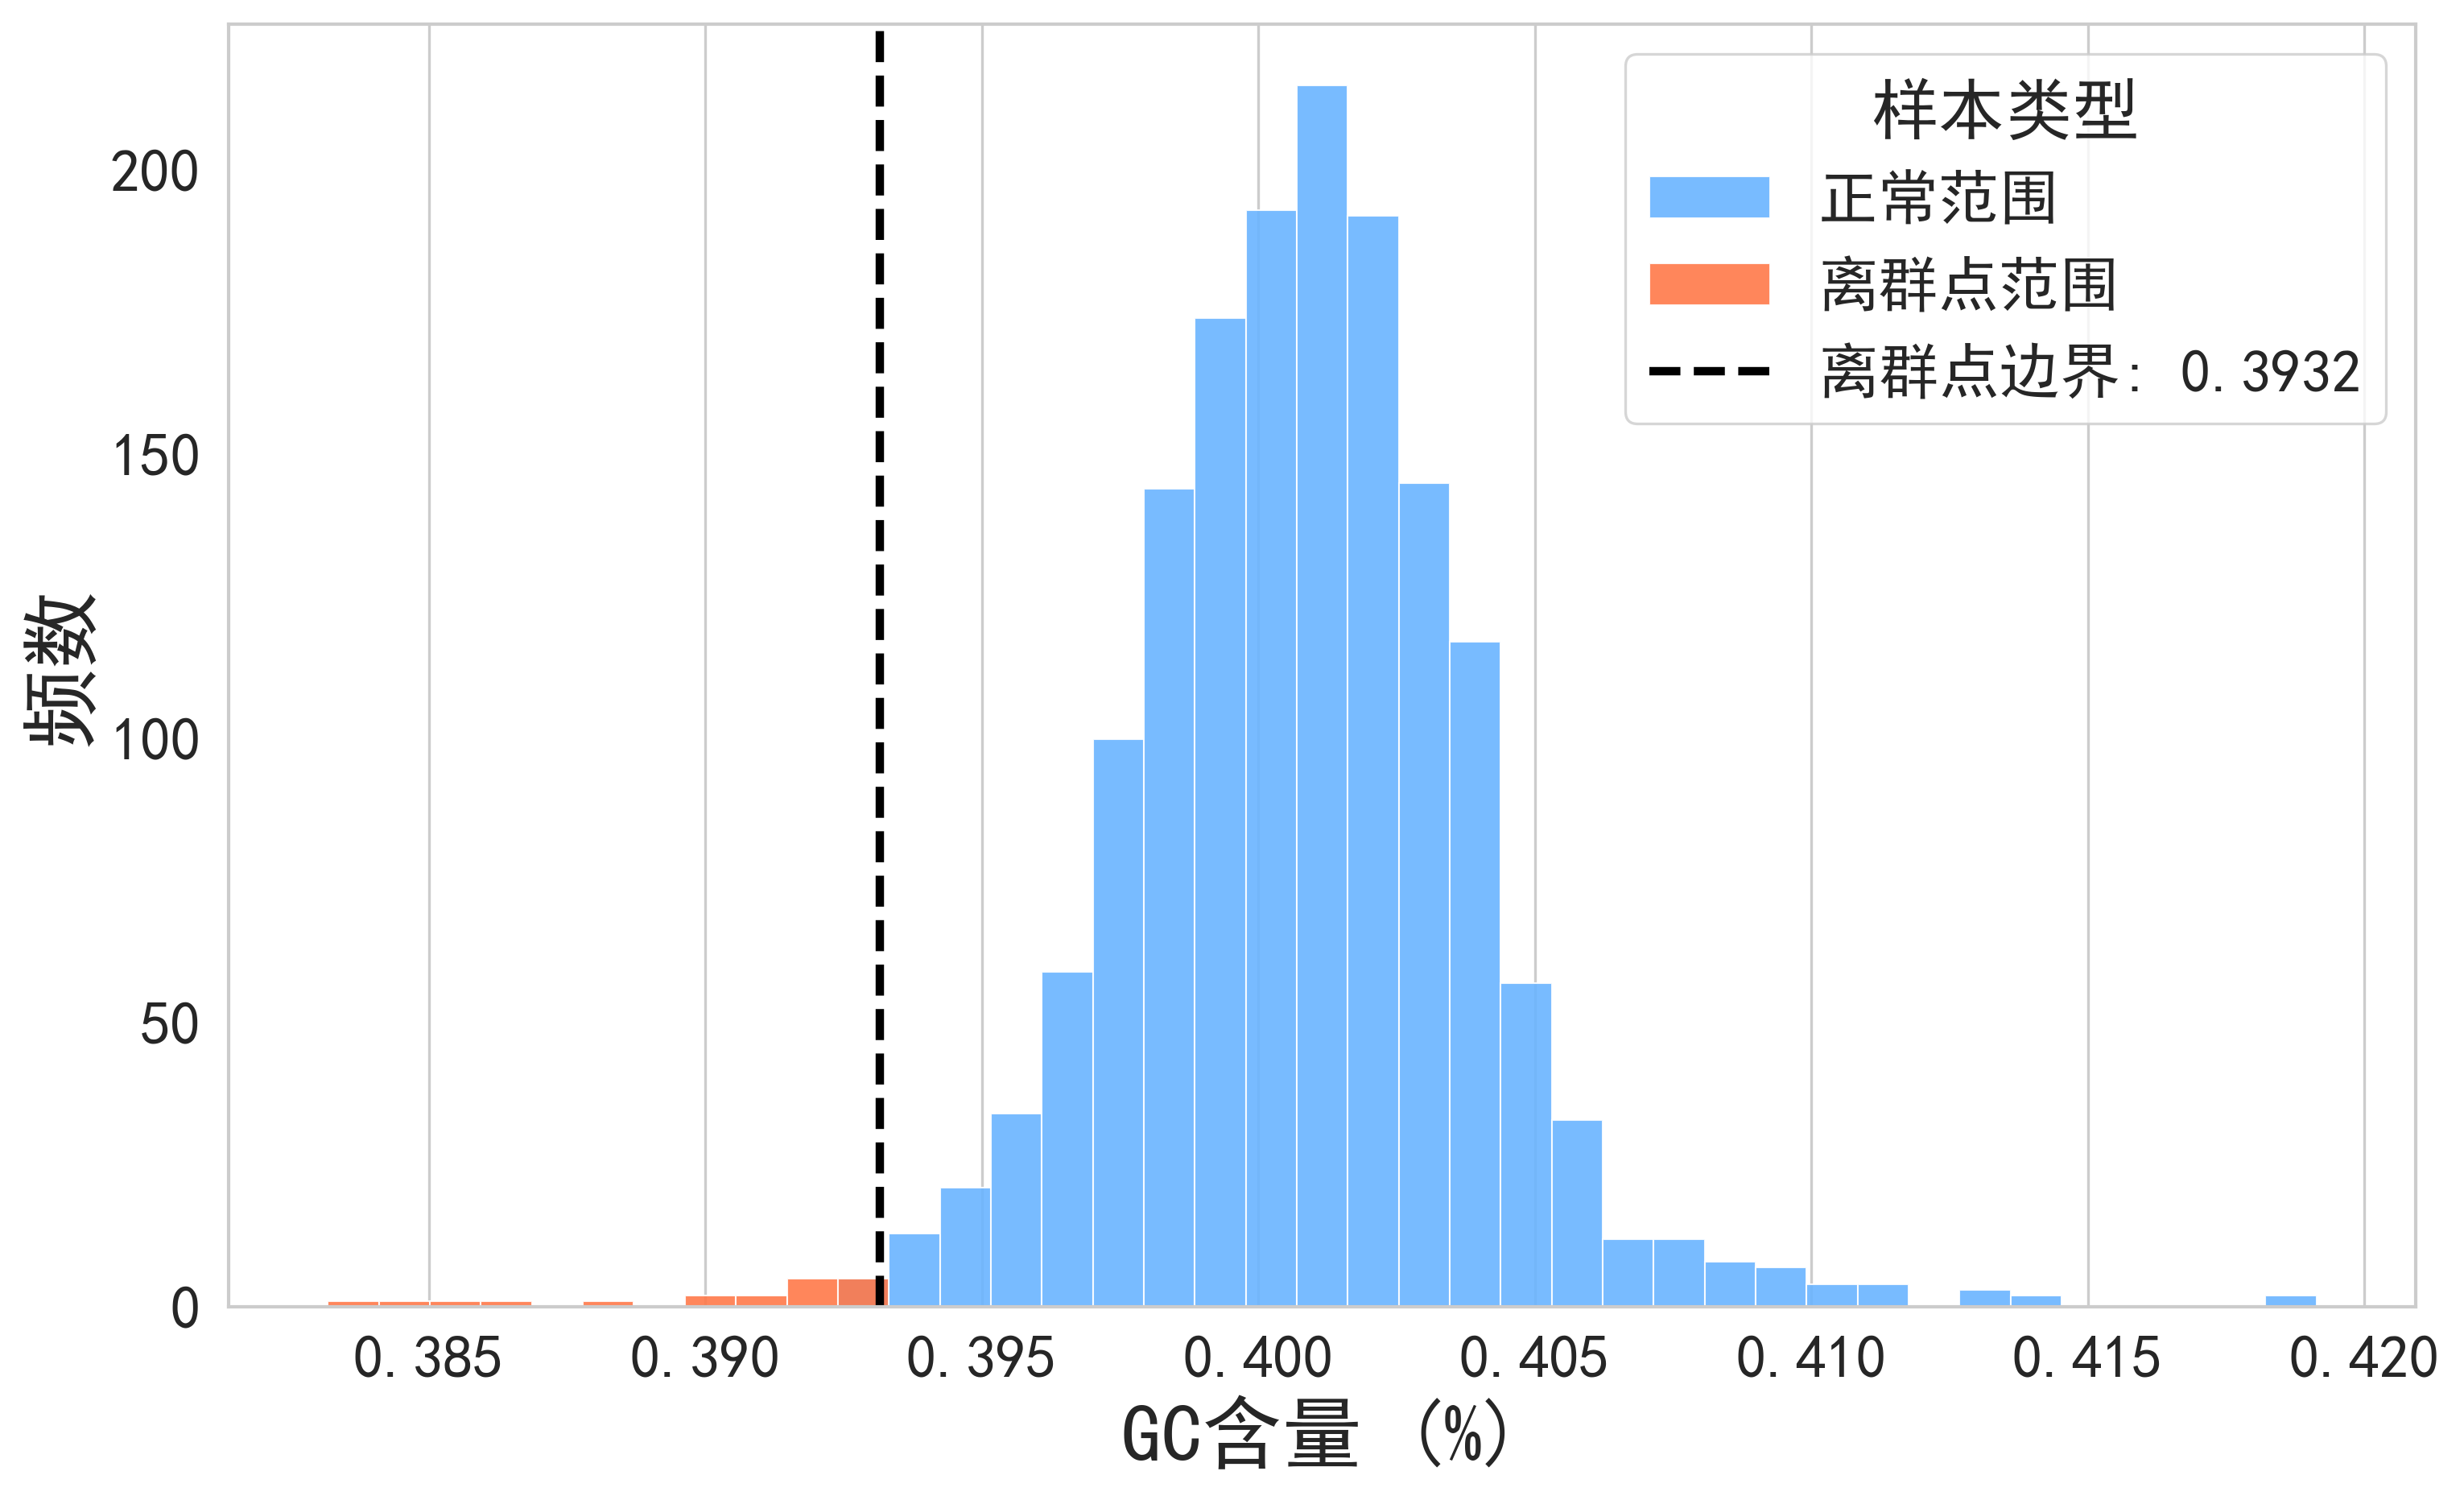
\includegraphics[width=\textwidth]{figs/2模型准备/图4_GC含量离群点分析.png}
\caption{GC含量离群点分析}
\label{fig:GC含量离群点分析}
\end{figure}

\subsection{数据量化}
为了便于后续相关数学模型的建立与求解,增强可理解性,我们进一步进行了数据量化。

针对不同问题,我们构建了相应的目标变量。对于男胎数据,依据题目定义的4\%阈值,我们创建了“Y浓度是否达标”的二元分类变量。对于女胎数据,则基于染色体的非整倍体列中空白即为无异常的定义,创建了“是否异常”以及各类异常的分类目标。\cref{fig:染色体异常类型分布}展示了女胎样本中正常与各类异常样本的数量分布。图中可见正常样本数量为488例,而18号,13号与21号染色体三体综合征的样本数量分别为45例,22例与13例。正常样本远多于异常样本,表明这是一个数据不平衡问题。

\begin{figure}[h!]
\centering
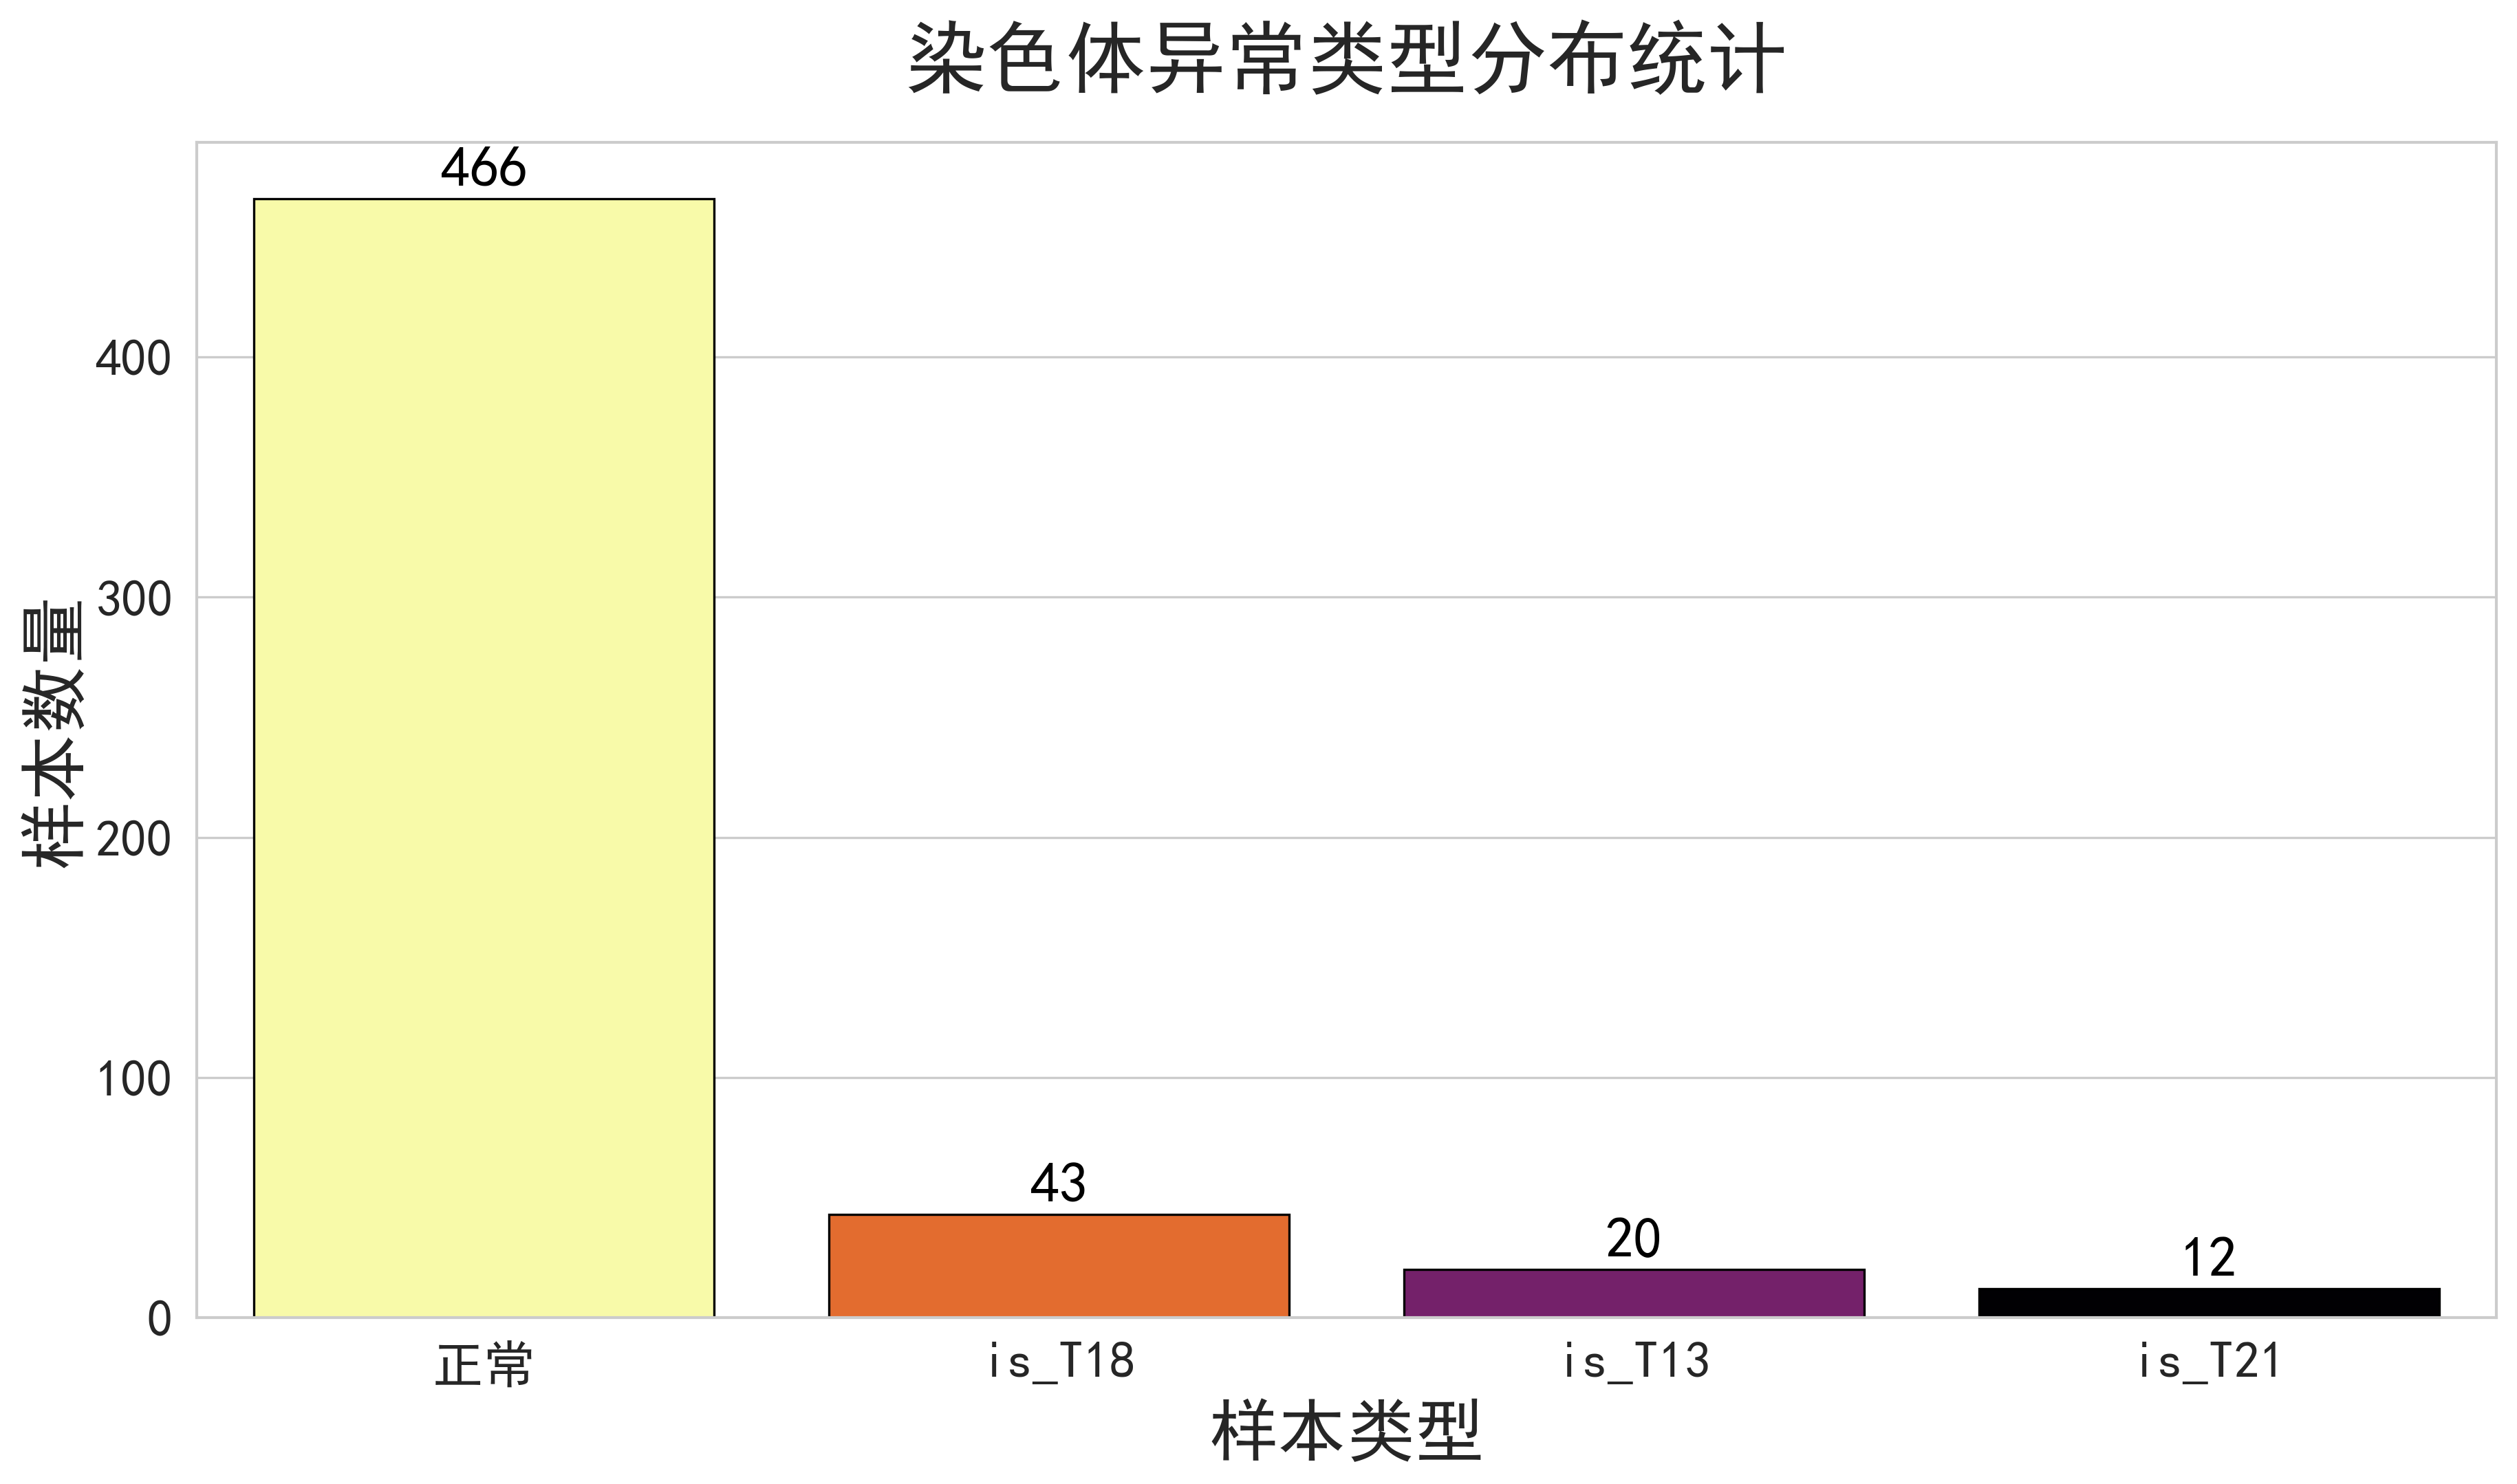
\includegraphics[width=0.8\textwidth]{figs/2模型准备/图5_染色体异常类型分布.png}
\caption{染色体异常类型分布}
\label{fig:染色体异常类型分布}
\end{figure}

考虑到问题四需要使用机器学习分类模型,我们仅针对女胎数据的所有数值型预测特征应用了标准化处理。标准化将所有特征转换到同一尺度,其计算方法如下
\begin{equation}
z = \frac{x - \mu}{\sigma}
\label{eq:standardization}
\end{equation}
其中 $x$ 为原始值,$\mu$ 为特征均值,$\sigma$ 为特征标准差。此操作避免了模型的训练过程被原始读段数等具有极大数值范围的特征所主导,使模型能够更稳定地学习所有特征的贡献。男胎数据因主要用于回归和优化分析,保留其原始数值的物理意义更为重要,故不进行缩放。\cref{fig:所有数值特征缩放效果对比}展示了女胎数据中所有数值型预测变量在缩放前后的分布对比。每个子图呈现了同一特征在处理前后的分布形态,处理前各变量的分布中心与尺度范围各不相同,而经过标准化处理后,所有变量的分布均被调整至以0为中心,具有相似的尺度,这为后续机器学习模型的训练提供了同质化的输入。

\begin{figure}[h!]
\centering
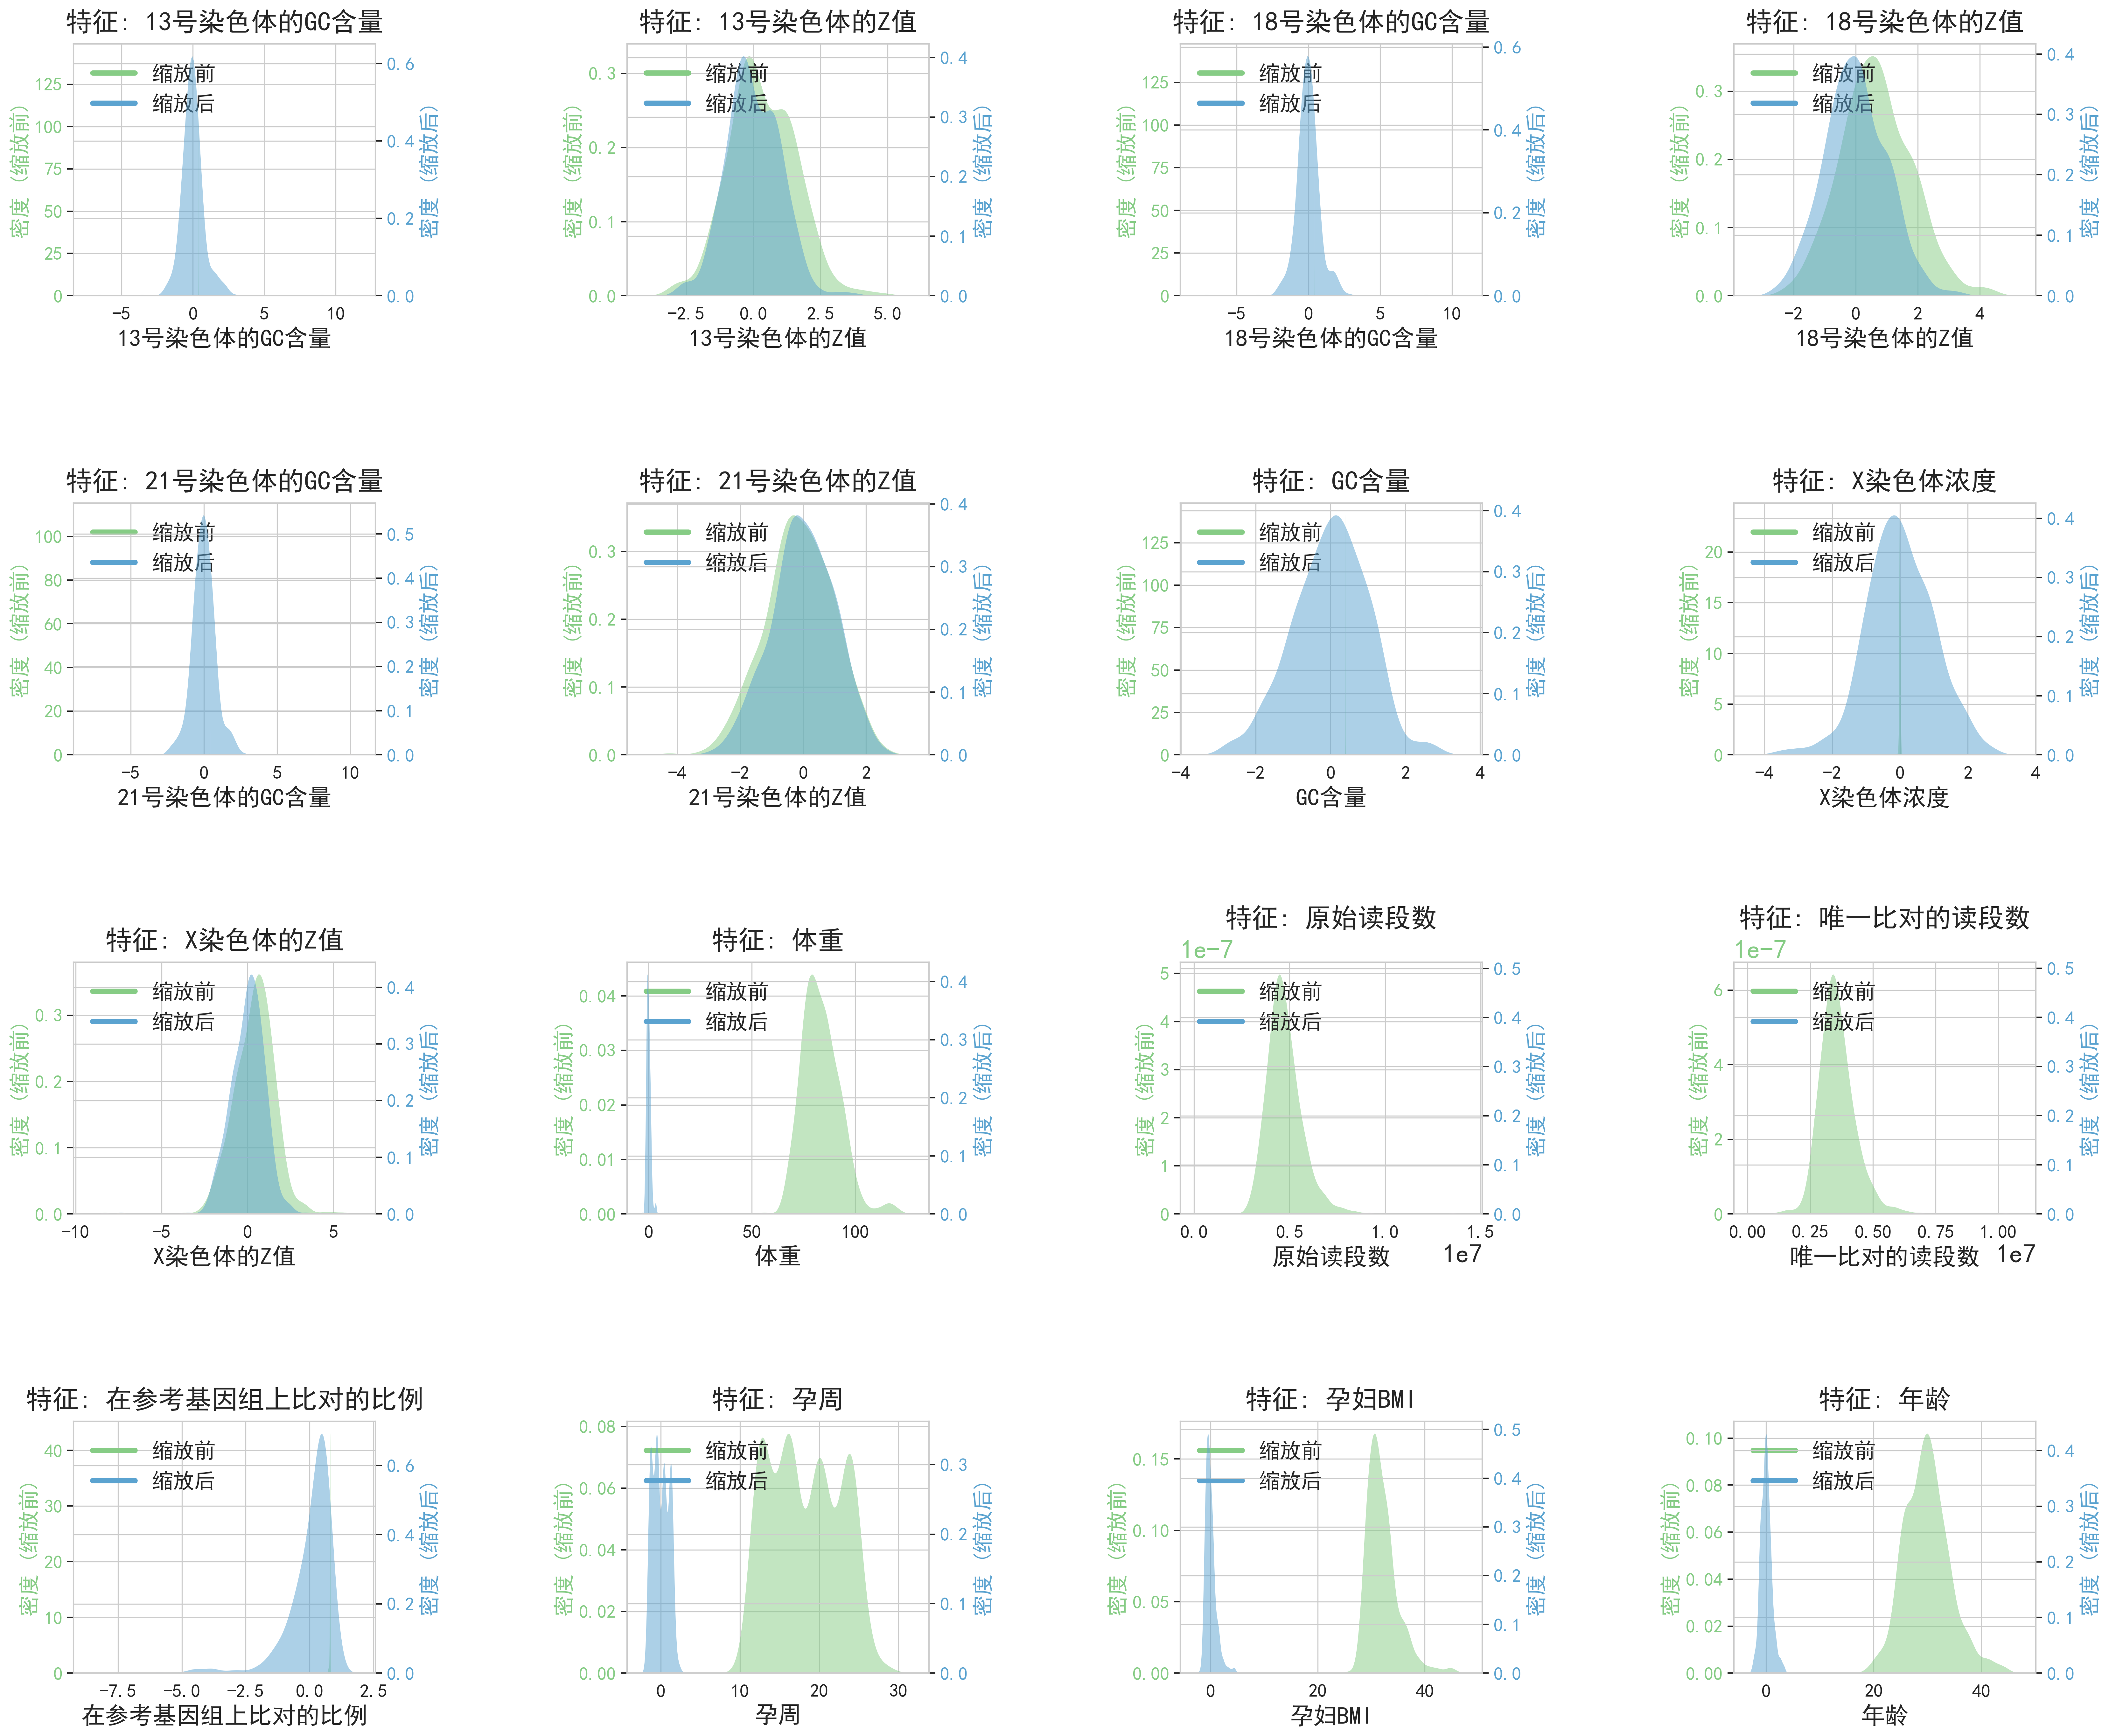
\includegraphics[width=1\textwidth]{figs/2模型准备/图6_特征缩放效果对比.png}
\caption{所有数值特征缩放效果对比}
\label{fig:数值特征缩放效果对比}
\end{figure}


此外,我们还构建了部分衍生特征。我们依据题目对风险的定义,创建了与孕周对应的风险等级特征。同时,为进行时序分析,还计算了每次检测距首次检测的天数。